\documentclass{article}
\usepackage{amsmath, amssymb, cite, algorithmic, url, braket}
\usepackage{graphicx}
\usepackage{pythonhighlight}
\usepackage[margin=1.5cm]{geometry}
\usepackage[title]{appendix}
\usepackage{subfigure}
\usepackage{listings}
\usepackage{booktabs}

\graphicspath{{../pic/}}
\lstset{
language=[ANSI]{C},
showtabs=true,
tab=,
tabsize=2,
basicstyle=\ttfamily\footnotesize,%\setstretch{.5},
stringstyle=\color{stringcolour},
showstringspaces=false,
alsoletter={1234567890},
otherkeywords={\%, \}, \{, \&, \|},
keywordstyle=\color{keywordcolour}\bfseries,
upquote=true,
morecomment=[s]{/*}{*/},
commentstyle=\color{commentcolour}\slshape,
literate=*%
{=}{{\literatecolour=}}{1}%
{-}{{\literatecolour-}}{1}%
{+}{{\literatecolour+}}{1}%
{*}{{\literatecolour*}}{1}%
{!}{{\literatecolour!}}{1}%
{[}{{\literatecolour[}}{1}%
{]}{{\literatecolour]}}{1}%
{<}{{\literatecolour<}}{1}%
{>}{{\literatecolour>}}{1}%
% {>>>}{\pythonprompt}{3}%
,%
frame=trbl,
rulecolor=\color{black!40},
backgroundcolor=\color{white},
breakindent=.5\textwidth,frame=single,breaklines=true
}

\begin{document}
\title{DSP Homework 08}
\author{Xu, Minhuan}
\maketitle
\tableofcontents
\begin{abstract}

\end{abstract}


\section{Comparison Between Two Sampling Methods}

\subsection{Local Adaptivity}
We can know from the class that the reconstructed function of the wan Sampling Method usually be like
\begin{equation}
	\hat{x}(t) = x(nT) + x'(nT)(t - nT) \quad T \in [n - \frac12, n + \frac12)
	\label{eq:WanReconstruct}
\end{equation}
Therefore, a certain time $\hat{x}(t)$ can be expressed only using near sampling points.

But, in the Shannon/Nyquist Sampling Method, we have derived the reconstructed function many times and that is
\begin{equation}
	x(t) = \sum_{n = - \infty}^{\infty} x(nT) \cdot sinc(\frac{t - nT}{T})
\end{equation}
That means for a certain point $t_0$ we have 
\begin{equation}
	x(t_0) = \sum_{n = - \infty}^{\infty} x(nT) \cdot \mathrm{sinc}(\frac{t_0 - nT}{T})
	\label{eq:SN-Recon}
\end{equation}
and this specific value is associated with all sampling points.

Therefore, if the receiver got a piece of signal from the sender, it's hard to determine the sampling rate in advance in Shannon/Nyquist Sampling Method. However, in Wan Sampling Method we can use (\ref{eq:WanReconstruct}) to sample this little piece of signal.

\subsection{Circuits}
In Shannon/Nyquist Sampling Method, see (\ref{eq:SN-Recon}), mathematical methods we must use are \emph{infinite} summation, multiple, sinc function. It is easy to find that the summation and the sinc function are difficult to implement.

In Wan Sampling Method, see (\ref{eq:WanReconstruct}), mathematical methods we must use are just \emph{finite} summation, multiple, differential calculus. In Analog Circuit, it is easy to do the plus, multiple, differential calculus using the operational amplifier.

\subsection{Flexible Error}
In Shannon/Nyquist Sampling Method, if we have determined the sampling rate in advance, the error is not predictable when the frequency of the signal is beyond the maximum frequency of Shannon/Nyquist Sampling Method.

In Wan Sampling Method, see subsection.\ref{wanSampling}, no matter what signal the receiver get, as long as we know the order of the reconstructed signal take, we can always find the maximum of the error. Moreover, if we take different order of the reconstructed signal,


\subsection{Flexible Bandwidth}
In Shannon/Nyquist Sampling Method, even there's only a little piece of the signal are relatively high-frequency, the sampling rate still should be set to the twice of the maximum frequency, otherwise there will be unpredictable error in the reconstructed function.

In Wan Sampling Method, because the reconstructed function $x(t)$ are only associated values within the interval of $[n - \frac12, n + \frac12)$. The signal bandwidth can be variable, which means we can choose wide-band channel when signal are wide-band, and choose narrow-band channel when signal are narrow band.

\subsection{My Understanding of Wan Sampling Method}
\label{wanSampling}

The Taylor Theorem is expressed as below.
$$
f(x) = \sum_{i = 0}^{N} ~ \frac{f^{(i)}(x_0)}{i!} ~ (x - x_0)^i + R_N(x)
$$

Applying to our signal $x(t)$, we can make $x_0 = nT, N = 2$ here and get the equation below. In this case, we assume that the value of $R_2(t)$ here is small enough compared with $\frac{x''(t_0)}{2}(x - t_0)^2$, so just ignore it.
\begin{equation}
	x(t) = x(nT) + x'(nT)(x - nT) + \frac{x''(t_0)}{2}(x - t_0)^2
\end{equation}


What exactly we get after sampling is only the values of $x(nT)$, but it is easy to do derivation. Therefore, using simple circuit, we know the values of $x'(nT),\,x''(nT),\,x'''(nT),\,\cdots$

So, the reconstructed signal $\hat{x}(t)$ can be expressed as
\begin{equation}
	x(t) = \overbrace{x(nT) + x'(nT)(x - nT)}^{\hat{x}(t)} + \frac{x''(t_0)}{2}(x - t_0)^2
\end{equation}
but also as
\begin{equation}
	x(t) = \overbrace{x(nT)}^{\hat{x}(t)} + x'(nT)(x - nT)
\end{equation}
The difference of the above two lies on the error of the reconstructed signal. It time to do the quantitative analysis, we assume that
\begin{equation}
	\begin{aligned}
		&|\hat{x}(t) - x(t)| &< \epsilon \\
		&|x^{(n)}(t)|  &< \eta_n \\ 
		&|x - nT|^n &< \frac{T}{2}
	\end{aligned}
\end{equation}
So, to ensure the accuracy, we need to make the sampling period $T$ satisfy the equations below.

\begin{equation}
	T < 2 \, \sqrt[n]{\frac{n! \,  \epsilon}{\eta_n}}
\end{equation}

About the value of $T$, I plotted a signal of $\cos(8t) + \sin(5t)\cos(2t)$ and the corresponding sampling period $T' = 2 \, \sqrt[n]{\frac{n!}{\eta_n}}$ ($\epsilon$ are ignored only to see the monotonicity of T about n), see Fig.~\ref{fig:maxes}.

\begin{figure}[!h]
	\centering
	\subfigure[Original Signal]{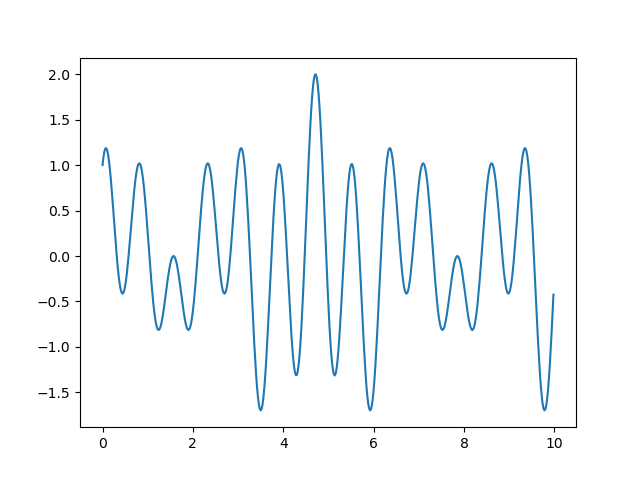
\includegraphics[height=2 in]{../pic/signal.png}}
	\hspace{0 pt}
	\subfigure[n - T']{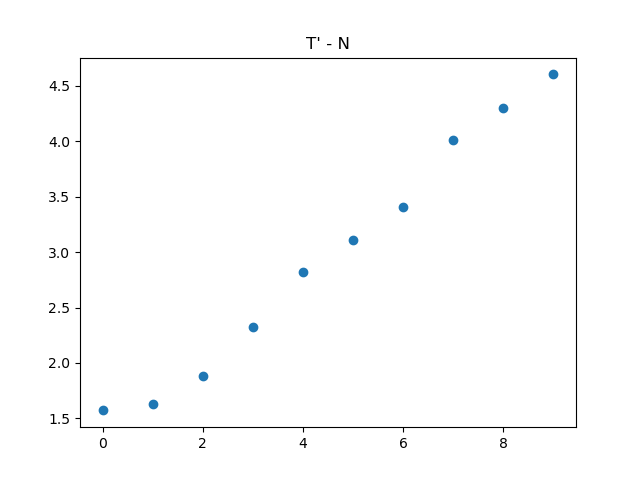
\includegraphics[height=2 in]{../pic/maxes.png }}
	\caption{The pictures I drew}
	\label{fig:maxes}
\end{figure}

Analyzing these digits, I found that with the same error $\epsilon$, if we raise the order of the $\hat{x}(t)$, the sampling rate can be set higher. In other words, it is the order of the reconstructed signal and the sampling rate decide the maximum of the error, and the two variables are negatively correlated when the error $\epsilon$ is fixed. So, if the accuracy is needed to be less, then what can be done is to raise the sampling rate or to raise the order of $\hat{x}(t)$.

\section{Conclusion}



\bibliographystyle{ieeetr}
\bibliography{../bib/database}

\begin{appendices}
\section{Code Listing}
\begin{python}
import numpy as np
from matplotlib import pyplot as plt

N = 10
t = np.arange(0, 20, 0.1)
func = np.cos(8*t)+np.sin(5*t)*np.cos(2*t)

fig1 = plt.figure()
plt.plot(t, func)
plt.show()

maxs = []
intv = [i for i in range(N)]

for i in range(1, N + 1):
    df = np.diff(func, i)
    df.resize(len(t))
    df /= (t[1] - t[0])**i
    nl = 1
    for j in range(1, i + 1):
        nl *= j
    maxs.append((nl/np.max(df))**(1/i))

fig2 = plt.figure()
plt.scatter(intv, maxs)
plt.show()
\end{python}
\end{appendices}

\end{document}